

\section{SQUISH-E Implementation}
The following sections focuses on the implementation of the elements described in the previous sections. In order to implement the algorithm, C was chosen because it allows the use of streaming technologies such as Kafka. It also allows the executable to be run at high speed because C is a compiled language, which reduces latency compared with other languages such as Python, which is an interpreted language, and Java, which runs on a Java Virtual Machine (JVM). The second advantage of this implementation choice is the use of the C language in database systems such as PostgreSQL in order to be able to implement the algorithm in MobilityDB.

In order to implement the SQUISH-E algorithm, it is necessary to follow the pseudo code and implement each component, as well as making certain implementation choices for elements that are not present in the C language. First SQUISH-E is a state-based algorithm. It does not return any output and have instead a state and update the state for each input. The output strategy chosen is like the sliding window where the last point are keep and the points are pushed into the database. 

\subsection{Algorithm 1 - SQUISH-E}

The first main loop is written as C function. The function have no return and changes the states of the variables.  This function take all the variables mentionned above it has some types and struct that will be described down. 

\begin{lstlisting}[float=ht,language=C, % Spécifie le langage du code
caption={Listing of the SQUISH-E algorithm implemented in C.}, % Légende du listing
label=lst:squish_c, % Étiquette pour référencer le listing
numbers=left,
numberstyle=\tiny\color{gray},
stepnumber=1,
frame=single,
breaklines=true,
postbreak=\mbox{\textcolor{red}{$\hookrightarrow$}\space},
showstringspaces=false
]
void
iteration_simplification_sqe(void *p_i , void *p_j ,
size_t *beta,const double lambda,int i,
Dict *succ,Dict *pred,
PDict  *p,struct PriorityQueue *Q,
bool syncdist,interpType interp ,bool hasz ,uint32_t minpts)
{
	if( i * lambda >= *beta)
	{
		*beta += 1;
	}
	set_priority_queue(p_i,INF,Q);
	set_priority_dict(p_i,0,p);
	if(i >= 1)
	{
		set_point_dict(p_i,p_j,pred);
		set_point_dict(p_j,p_i,succ);
		adjust_priority(p_j,Q,pred,succ,p, syncdist, interp , hasz );
	}
	size_t size = size_queue(Q);
	if(size - *beta == 0 ){
		reduce(Q,pred,succ,p,syncdist, interp , hasz );
	}
}
\end{lstlisting}


The algorithm in Listing \ref{lst:squish_c} follows the pseudo code of SQUISH-E. It utilizes the set function for the priority queue, as well as the set functions for the point map and priority map, which will be described in the implementation section. The reduce function and adjust priority functions are called to manage the size of the data structure when it meets the threshold. These functions also adjust the priority for each point that has both a predecessor and a successor, in order to calculate the error that would result from removing the corresponding point.

\subsection{Algorithm 2 - Reduce}
Then we have the main block of SQUISH-E, which is the reduce part.



\begin{lstlisting}[language=C, % Spécifie le langage du code
caption={Implementation of the reduce function in C.}, % Légende du listing
label=lst:reduce_c, % Étiquette pour référencer le listing
numbers=left,
numberstyle=\tiny\color{gray},
stepnumber=1,
frame=single,
breaklines=true,
postbreak=\mbox{\textcolor{red}{$\hookrightarrow$}\space},
showstringspaces=false,
float,
floatplacement=H
]
void
reduce(struct PriorityQueue *Q,Dict *pred,Dict *succ,PDict  *p,
bool syncdist,interpType interp ,bool hasz )
{
	struct PriorityQueueElem *entry = remove_min(Q);
	size_t size_before = size_queue(Q);
	
	void * p_j = entry->point;
	double priority = entry->priority;
	
	void * p_i = get_point_dict(p_j,pred);
	void * p_k = get_point_dict(p_j,succ);
	
	double pr_i = get_priority_dict(p_i,p); if(priority > pr_i){ pr_i = priority; }
	double pr_k = get_priority_dict(p_k,p); if(priority > pr_k){ pr_k = priority; }
	
	set_priority_dict(p_k, pr_k ,p);
	set_priority_dict(p_i, pr_i ,p);
	
	set_point_dict(p_i,p_k,succ);
	set_point_dict(p_k,p_i,pred);
	set_point_dict(p_k,p_i,pred);
	
	adjust_priority(p_k ,Q,pred,succ,p,syncdist, interp ,hasz );
	adjust_priority(p_i ,Q,pred,succ,p,syncdist, interp ,hasz );
	
	
	//Delete pointer
	free(entry);
	destroy_elem_PriorityDict(p_j,p);
	destroy_elem_PointDict(p_j,succ);
	destroy_elem_PointDict(p_j,pred);
}

\end{lstlisting}

This algorithm in Listing \ref{lst:reduce_c} describes the reduction method. As mentioned above, it removes the lowest priority points from the queue and updates the neighbors. Since we use the C language, we free the memory of the unnecessary data. Each call is represented by a function to simplify implementation and break it down into manageable pieces of code for each particular variable. This choice of implementation also allows for flexibility in changing the structure.

\subsection{Algorithm 3 - Adjust Priority} 

\begin{lstlisting}[language=C, % Spécifie le langage du code
caption={C code implementation of the adjust\_priority function.}, % Légende du listing
label=lst:adjust_c, % Étiquette pour référencer le listing
numbers=left,
numberstyle=\tiny\color{gray},
stepnumber=1,
frame=single,
breaklines=true,
postbreak=\mbox{\textcolor{red}{$\hookrightarrow$}\space},
showstringspaces=false,
float,
floatplacement=H
]
void
adjust_priority(void *p_i,struct PriorityQueue *Q, Dict *pred,Dict *succ,PDict  *p,
bool syncdist,interpType interp ,bool hasz )
{
	void * p_h = get_point_dict(p_i,pred);
	void * p_k = get_point_dict(p_i,succ);
	if( p_h != NULL &&  p_k != NULL )
	{
		if(syncdist)
		{
			double priority = get_priority_dict(p_i,p) + SED(p_h,p_i,p_k, interp , hasz );
			set_priority_queue(p_i,priority,Q);
		}
	}
}

\end{lstlisting}
 

The algorithm in Listing \ref{lst:adjust_c} highlights what differentiates SQUISH from SQUISH-E. When a point is removed, the surrounding points are updated, and their priorities are adjusted accordingly. This process involves retrieving the neighboring points and recalculating their priorities based on the previously stored error in the dictionary and the synchronized Euclidean distance calculation.


\section{Variables Implementation}
In this section, we will discuss how the variables have been implemented and evaluate their effectiveness. This will be followed by a discussion on the performance and complexity achieved.


\subsection{Map}
In this section, we will focus on the implementation of the map.


\begin{lstlisting}[float=ht,language=C, % Spécifie le langage du code
caption={C code implementation of the Map data structure.}, % Légende du listing
label=lst:map_c, % Étiquette pour référencer le listing
numbers=left,
numberstyle=\tiny\color{gray},
stepnumber=1,
frame=single,
breaklines=true,
postbreak=\mbox{\textcolor{red}{$\hookrightarrow$}\space},
showstringspaces=false
]
#include <search.h>

typedef struct PriorityDict
{
void * key;
double priority;
} PriorityDict;


typedef struct PointDict
{
void *key;
void *value;
} PointDict;


typedef void* Dict;
typedef void* PDict;
\end{lstlisting}
 

This structure in Listing \ref{lst:map_c} represents a Map that links a point to a corresponding value, such as a priority or another point. We define a struct with two fields: the key and the value. The \texttt{typedef void*} is used for the GNU Library to avoid using \texttt{void**}, adding more clarity to the code.


\paragraph{Method}

\begin{lstlisting}[float=ht,language=C, % Spécifie le langage du code
caption={Methods get\_point for the Map implementation in C.}, % Légende du listing
label=lst:pmap_c_g, % Étiquette pour référencer le listing
numbers=left,
numberstyle=\tiny\color{gray},
stepnumber=1,
frame=single,
breaklines=true,
postbreak=\mbox{\textcolor{red}{$\hookrightarrow$}\space},
showstringspaces=false
]
void *
get_point_dict(void *p_i,Dict *dict)
{
	PointDict find;
	find.key = p_i;
	void * result = tfind(&find, dict, compar);
	if(result){
		result = (*(PointDict**)result)->value;
	}
	return result;
}

\end{lstlisting} 

\begin{lstlisting}[float=ht,language=C, % Spécifie le langage du code
caption={Methods set\_point for the Map implementation in C.}, % Légende du listing
label=lst:pmap_c_s, % Étiquette pour référencer le listing
numbers=left,
numberstyle=\tiny\color{gray},
stepnumber=1,
frame=single,
breaklines=true,
postbreak=\mbox{\textcolor{red}{$\hookrightarrow$}\space},
showstringspaces=false
]
void
set_point_dict(void * p_i,void * p_j,Dict *dict)
{
	PointDict *find = malloc(sizeof(PointDict));
	find->key = p_i;
	find->value = p_j;
	void * result = tfind(find, dict, compar);
	if(result){
		(*(PointDict**)result)->value = p_j;
	}
	else{
		tsearch(find, dict, compar); /* insert */
	}
}
\end{lstlisting} 


\begin{lstlisting}[float=ht,language=C, % Spécifie le langage du code
caption={Methods destroy\_elem for the Map implementation in C.}, % Légende du listing
label=lst:pmap_c, % Étiquette pour référencer le listing
numbers=left,
numberstyle=\tiny\color{gray},
stepnumber=1,
frame=single,
breaklines=true,
postbreak=\mbox{\textcolor{red}{$\hookrightarrow$}\space},
showstringspaces=false
]
void destroy_elem_PointDict(void * p_i,Dict *dict)
{
	PointDict find;
	find.key = p_i;
	void * r = tfind(&find, dict, compar);
	if(r)
	{
		PointDict * to_free = (*(PointDict**)r);
		tdelete(&find,dict,compar);
		free(to_free);
	}
}

\end{lstlisting} 

In the Listings \labelcref{lst:pmap_c,lst:pmap_c_g,lst:pmap_c_s}, we utilize functions from the GNU C Library that implement a binary tree. This structure ensures that each operation has a maximum complexity of \( O(\log(n)) \). Both mappings use the same implementation. Ideally, it would be beneficial to resolve this duplication by using a template or a similar approach, but the capabilities of the C language impose certain limitations.


\paragraph{Discussion}
As mentioned in the previous subsection, the map uses the GNU C Library binary tree structure to perform search and set operations. These algorithms have a complexity of \( O(\log(n)) \) and feature dynamic memory allocation.

\subsection{PriorityQueue}

\begin{lstlisting}[float=ht,language=C, % Spécifie le langage du code
caption={C code implementation of the PriorityQueue.}, % Légende du listing
label=lst:prqueue_c, % Étiquette pour référencer le listing
numbers=left,
numberstyle=\tiny\color{gray},
stepnumber=1,
frame=single,
breaklines=true,
postbreak=\mbox{\textcolor{red}{$\hookrightarrow$}\space},
showstringspaces=false
]
typedef struct PriorityQueueElem
{
	void * point;
	double priority;
	int index; //reference his own index
} PriorityQueueElem;

typedef void* IDict;

typedef struct PriorityQueue
{
	PriorityQueueElem **arr;
	IDict dict;
	size_t size;
	size_t capacity;
} PriorityQueue;

\end{lstlisting} 

This structure in Listing \ref{lst:prqueue_c} implements the functions of a priority queue using the structure of a min heap. It uses a `PriorityQueueElem` which contains the point, the corresponding priority, and a reference to this index in the heap. The main structure uses an array of pointers to `PriorityQueueElem`, along with an index map, an integer representing the number of points in the queue, and finally, the number of points allocated.


\paragraph{Method}

After establishing the algorithm's framework, the next step is to implement the methods for the described variables to complete the implementation process.

\begin{lstlisting}[float=ht,language=C, % Spécifie le langage du code
	caption={C code implementation of the PriorityQueue's Remove Min function.}, % Légende du listing
	label=lst:prqueueMethodR_c, % Étiquette pour référencer le listing
	numbers=left,
	numberstyle=\tiny\color{gray},
	stepnumber=1,
	frame=single,
	breaklines=true,
	postbreak=\mbox{\textcolor{red}{$\hookrightarrow$}\space},
	showstringspaces=false
]	
PriorityQueueElem *remove_min(PriorityQueue *Q)
{
	PriorityQueueElem *result = NULL;
	if (Q->size != 0) {
		result = Q->arr[0];
		// Replace the deleted node with the last node
		Q->arr[0] = Q->arr[Q->size - 1];
		Q->arr[Q->size - 1] = NULL;
		if(Q->arr[0]){
			Q->arr[0]->index = 0;
		}
		
		// Decrement the size of heap
		Q->size--;
		
		tdelete(result,&Q->dict,compar_index);
		// Call minheapify_top_down for 0th index
		// to maintain the heap property
		minHeapify(Q, 0);
	}
	return result;
}
\end{lstlisting}


To remove the point with the minimum result, we employ the procedure outlined in Listing \ref{lst:prqueueMethodR_c}: First, we verify the number of elements and retrieve the first one. Our insertion methods guarantee that this first element always holds the minimum result. Next, we extract the last element, relocate it to the beginning of the queue, and rebalance the tree to maintain the smallest element at index 0. Finally, we remove the index from the dictionary.

\begin{lstlisting}[float=ht,language=C, % Spécifie le langage du code
caption={C code implementation of the PriorityQueue's Set Priority function.}, % Légende du listing
label=lst:prqueueMethodSet_c_s, % Étiquette pour référencer le listing
numbers=left,
numberstyle=\tiny\color{gray},
stepnumber=1,
frame=single,
breaklines=true,
postbreak=\mbox{\textcolor{red}{$\hookrightarrow$}\space},
showstringspaces=false
]
void
set_priority_queue(void *p_i,double priority ,PriorityQueue *Q)
{
	struct PriorityQueueElem * insert = replace_elem(p_i,priority,Q);
	if(insert == NULL){
		insert = malloc(sizeof(struct PriorityQueueElem));
		insert->point = p_i;
		insert->priority = priority;
		insert->index = -1;
		tsearch(insert, &Q->dict, compar_index); /* insert */
	}
	if(insert->index == -1){
		push(insert,Q);
	}
}
\end{lstlisting}

\begin{lstlisting}[float=ht,language=C, % Spécifie le langage du code
caption={C code implementation of the PriorityQueue's Replace elem function.}, % Légende du listing
label=lst:prqueueMethodSet_c_r, % Étiquette pour référencer le listing
numbers=left,
numberstyle=\tiny\color{gray},
stepnumber=1,
frame=single,
breaklines=true,
postbreak=\mbox{\textcolor{red}{$\hookrightarrow$}\space},
showstringspaces=false
]
struct PriorityQueueElem *
replace_elem(void *p_i,double priority ,PriorityQueue *Q)
{
	PriorityQueueElem *elem = get_elem(p_i,&Q->dict);
	if(elem ){
		if(Q->size > elem->index && elem->index != -1){
			Q->arr[elem->index]->priority = priority;
			insertHelper(Q, elem->index);
			minHeapify(Q, elem->index);
		}
	}
	return elem;
}
\end{lstlisting}

\begin{lstlisting}[float=ht,language=C, % Spécifie le langage du code
caption={C code implementation of the PriorityQueue's Push function.}, % Légende du listing
label=lst:prqueueMethodSet_c, % Étiquette pour référencer le listing
numbers=left,
numberstyle=\tiny\color{gray},
stepnumber=1,
frame=single,
breaklines=true,
postbreak=\mbox{\textcolor{red}{$\hookrightarrow$}\space},
showstringspaces=false
]
void
push(PriorityQueueElem * insert,PriorityQueue *Q)
{
	Q->size++;
	if(Q->size > Q->capacity){
		Q->arr = realloc(Q->arr, Q->size * sizeof(PriorityQueueElem*));
	}
	Q->arr[Q->size-1] = insert;
	Q->arr[Q->size-1]->index = Q->size-1;
	insertHelper(Q, Q->size-1);
}

\end{lstlisting}

In other implementations, the procedures detailed in Listings \labelcref{lst:prqueueMethodSet_c_s,lst:prqueueMethodSet_c_r,lst:prqueueMethodSet_c} are designed with a maximum complexity of $O(\log(n))$. The decision to utilize a min heap structure for implementing the priority queue aligns with this complexity constraint established during the design phase.

A min heap, as illustrated in Figure \ref{fig:min_heap}, embodies a tree-like structure where each node adheres to the property that parent nodes are always smaller than their child nodes. This property ensures efficient retrieval of the minimum element.

The min heap implementation is derived from a reference on the website \footnote{https://www.geeksforgeeks.org/c-program-to-implement-min-heap/}, providing inspiration for its construction.


\begin{figure}[!h]
\centering
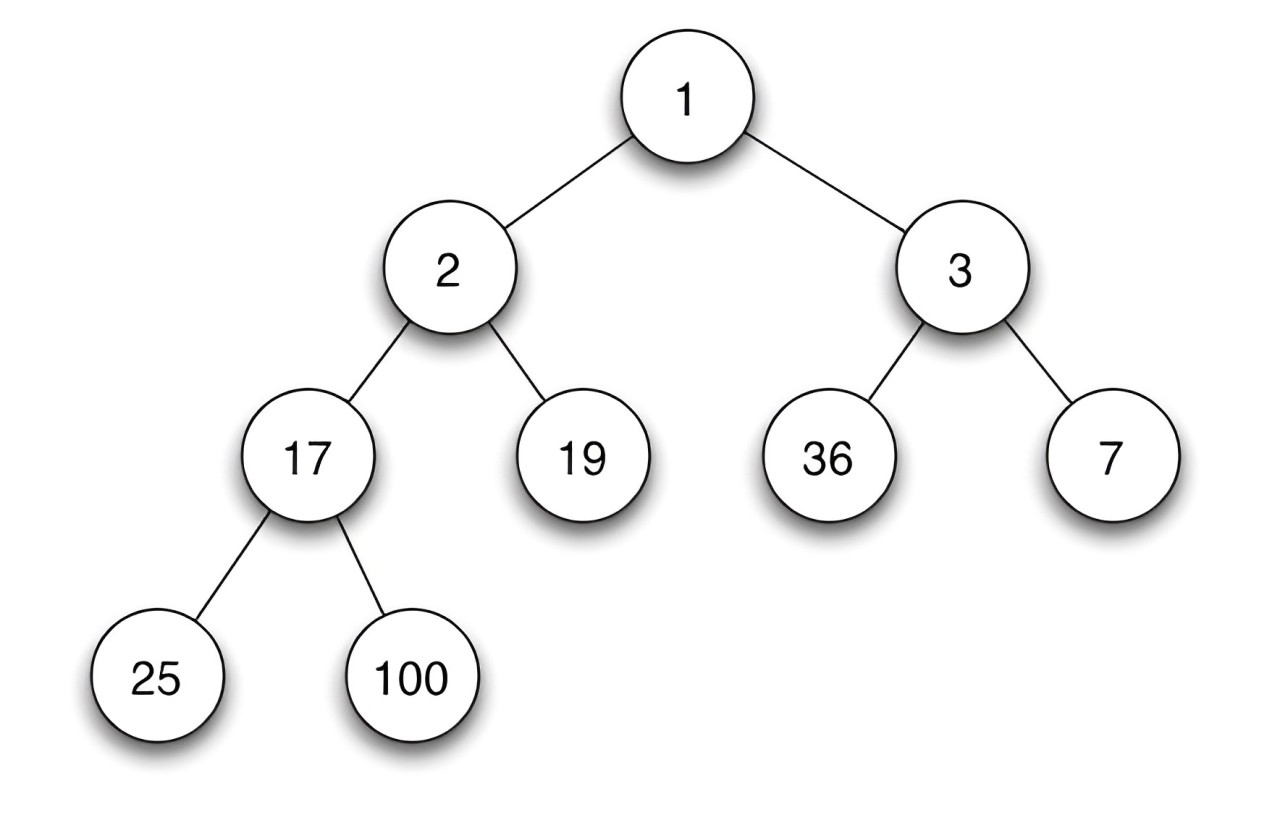
\includegraphics[width=1\linewidth]{figures/tree.jpeg}
\caption{Illustration of the Min Heap structure.}
\label{fig:min_heap}
\end{figure}


\paragraph{Discussion}

The concept here revolves around leveraging the min heap structure to achieve a maximum complexity of $O(\log(n))$ for obtaining the point with the lowest priority. Additionally, an index map is utilized to facilitate efficient replacement of points within the heap. This approach benefits from static memory allocation, a desirable trait.
The set employs mapping to determine if a point is already present in the map. If it is, the point's priority is adjusted within the heap, followed by checks with its ancestors and descendants to maintain the min heap property. If the point is not present, it is added to the end of the heap, and adjustments are made to satisfy the min heap condition.
Ultimately, both operations required by the algorithm achieve a complexity of $O(\log(n))$, ensuring efficient performance.

\section{PostgreSQL Implementation}

In this section, we detail the implementation of the algorithm within the MobilityDB SQL functions.

\subsection{SQL Code}
As the implementation is in C, the SQL code provided in Listing \ref{lst:squish_SQL} serves solely as a reference to the corresponding C function.\\

\begin{lstlisting}[
language=SQL, % Setting the language for SQL
caption={SQL code implementing the SQUISH-E algorithm.}, % Caption for the listing
float=ht,
label=lst:squish_SQL, % Label for referencing the listing
basicstyle=\ttfamily\small, % Basic style
keywordstyle=\color{blue}\ttfamily, % Style for keywords
stringstyle=\color{red}\ttfamily, % Style for strings
commentstyle=\color{green}\ttfamily, % Style for comments
numbers=left, % Line numbers on the left
numberstyle=\tiny\color{gray}, % Style for line numbers
stepnumber=1, % Line numbers step
frame=single,
breaklines=true, % Automatic line breaking
postbreak=\mbox{\textcolor{red}{$\hookrightarrow$}\space}, % Arrow for line breaks
showstringspaces=false % Don't show special spaces within strings
]
CREATE FUNCTION SquishESimplify(tfloat, float, boolean DEFAULT TRUE)
RETURNS tfloat
AS 'MODULE_PATHNAME', 'Temporal_simplify_sqe'
LANGUAGE C IMMUTABLE STRICT PARALLEL SAFE;
CREATE FUNCTION SquishESimplify(tgeompoint, float, boolean DEFAULT TRUE)
RETURNS tgeompoint
AS 'MODULE_PATHNAME', 'Temporal_simplify_sqe'
LANGUAGE C IMMUTABLE STRICT PARALLEL SAFE;
\end{lstlisting}

\subsection{Example}
This section presents examples demonstrating the usage of the PostgreSQL function described in Listing \ref{lst:squish_SQL}. These examples illustrate how the algorithm can be utilized in offline settings using queries.\\


\begin{lstlisting}[
language=SQL, % Setting the language for SQL
float=ht,
caption={Example SQL queries demonstrating the use of the SQUISH-E algorithm.}, % Caption for the listing
label=lst:example_SQL, % Label for referencing the listing
basicstyle=\ttfamily\small, % Basic style
keywordstyle=\color{blue}\ttfamily, % Style for keywords
stringstyle=\color{red}\ttfamily, % Style for strings
commentstyle=\color{green}\ttfamily, % Style for comments
numbers=left, % Line numbers on the left
numberstyle=\tiny\color{gray}, % Style for line numbers
stepnumber=1, % Line numbers step
frame=single,
breaklines=true, % Automatic line breaking
postbreak=\mbox{\textcolor{red}{$\hookrightarrow$}\space}, % Arrow for line breaks
showstringspaces=false % Don't show special spaces within strings
]
SELECT SquishESimplify(tfloat '[1@2000-01-01, 2@2000-01-02, 3@2000-01-04,
4@2000-01-05]', '1 day');
-- [1@2000-01-01, 3@2000-01-04]

SELECT asText(SquishESimplify(tgeompoint '[Point(1 1 1)@2000-01-01,
Point(2 2 2)@2000-01-02, Point(3 3 3)@2000-01-04, Point(5 5 5)@2000-01-05)', 0.5));
-- [POINT Z (1 1 1)@2000-01-01, POINT Z (3 3 3)@2000-01-04,POINT Z (5 5 5)@2000-01-05)

\end{lstlisting}
